%----------------------------------------------------------------------------------------
%	ABSTRACT
%----------------------------------------------------------------------------------------
\initial{Ο}{\color{teal}ι διεργασίες είναι τα προγράμματα που εκτελούνται, τα οποία πρέπει να μάθουμε να τα διαχειριζόμαστε: να τα σταματάμε, να τα τερματίζουμε και να τους στέλνουμε σήματα.
Οι μεταβλητές χρησιμοποιούνται είτε από το φλοιό είτε από άλλα προγράμματα, όπως τα shell scripts είτε για παραμετροποίηση του περιβάλλοντος εργασίας είτε για αποθήκευση τιμών. Υπάρχουν οι τοπικές μεταβλητές και οι μεταβλητές περιβάλλοντος.}

\epigraphhead[10]{\epigraph{"The UNIX legacy is a set of simple and timeless tools that can take years to master but which can perform seeming miracles in seconds in the hands of experienced users. "}{\textit{\href{http://www.linfo.org/index.html}{http://www.linfo.org/index.html}}}}

%----------------------------------------------------------------------------------------
%	ARTICLE CONTENTS
%----------------------------------------------------------------------------------------

\section{Διεργασίες}

\begin{figure}[ht]
	\centering
	%\scalebox{0.2}{\includegraphics{unix-tree.eps}}
	%\resizebox{\linewidth}{!}{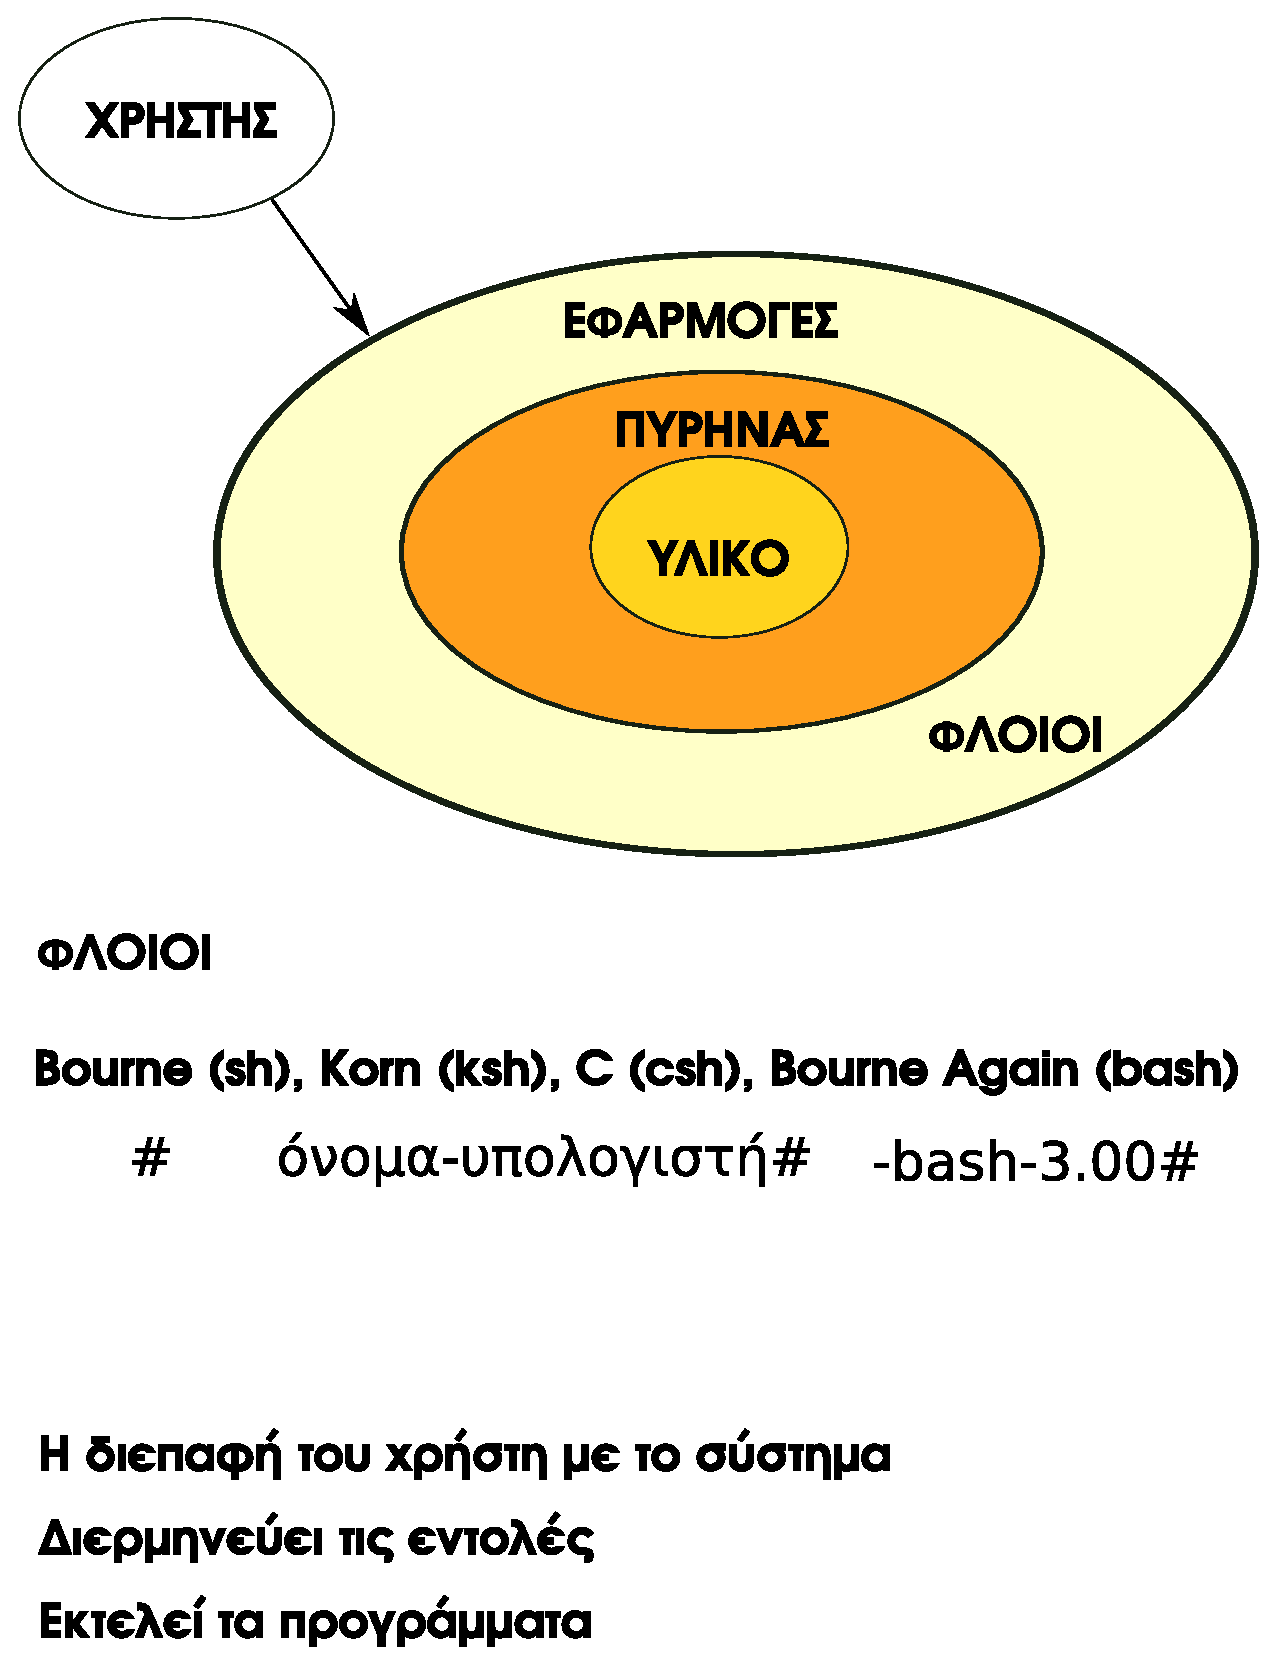
\includegraphics{shells.eps}}
	\scalebox{0.55}{\includegraphics{images/process_states.jpg}}
	\caption{Καταστάσεις διεργασιών}
	\label{fig:process-states}
\end{figure} 

Η διεργασία είναι ένα πρόγραμμα που εκτελείται. Η διεργασία έχει πολλά συστατικά  μέρη και ιδιότητες. Ανάμεσα σε αυτές είναι το PID (process
identity – ταυτότητα διεργασίας), προτεραιότητα και κάποια άλλα. Κάθε διεργασία, εκτός από την init, δημιουργείται από κάποια άλλη. Κάθε
διεργασία μπορεί να δημιουργήσει και άλλες. Η διεργασία init\footnote{\href{https://docs.oracle.com/cd/E23823\_01/html/817-0403/glybe.html}{https://docs.oracle.com/cd/E23823\_01/html/817-0403/glybe.html}}, η οποία είναι η πρώτη διεργασία του συστήματος και δημιουργείται κατά την
εκκίνηση του συστήματος (boot), έχει πάντα PID 1. Μία διεργασία μπορεί να έχει ταυτόχρονα και «γονέα» (parent) και «παιδί» (child). Η εντολή
\textbf{tree} (Linux) ή \textbf{ptree} (Solaris) εμφανίζει το δέντρο όλων των διεργασιών του συστήματος.

Η εντολή \textbf{ps} εμφανίζει πληροφορίες για τις διεργασίες που εκτελούνται.  Χωρίς παραμέτρους εμφανίζει τις διεργασίες που αντιστοιχούν
στο συγκεκριμένο τερματικό. Σημαντικοί παράμετροι της εντολής είναι:

\begin{packed_item}
	\item   \textbf{-a}, εμφανίζει όλες τις διεργασίες, δεν περιλαμβάνονται οι διεργασίες που δεν ελέγχονται από συγκεκριμένο τερματικό.
	\item   \textbf{-e}, εμφανίζει όλες τις διεργασίες
	\item   \textbf{-u username}, εμφανίζει τις διεργασίες του χρήστη 
\end{packed_item}

Δεδομένου ότι σε ένα σύστημα Unix μπορεί να εκτελούνται εκατοντάδες διεργασίες, μία συνήθης τεχνική για να βρούμε αν εκτελείται μία
συγκεκριμένη διεργασία είναι η χρήση της \textbf{ps} μαζί με την \textbf{grep}, \textbf{ps -a | grep 'bash'}. Αν η παραπάνω εντολή
επιστρέψει μία μόνο γραμμή (που είναι η εντολή που μόλις δώσαμε), τότε η διεργασία bash δεν εκτελείται.Αν θέλετε μία λίστα διεργασιών που
ανανεώνεται συνεχώς, χρησιμοποιήστε την εντολή \textbf{prstat}\footnote{H prstat λειτουργεί στο Solaris, ενώ στο linux η αντίστοιχη είναι η top}. Η top είναι αρκετά εύχρηση εντολή και μπορούμε να φιλτράρουμε τις διεργασίες ανάλογα με κάποιες παραμέτρους. Επίσης υπάρχει και η εντολή htop (δεν είναι εγκατεστημένη εκ των προτέρων στα συστήματα) η οποία μας δείχνει και σε διάγραμμα κάποια στατιστικά των διεργασιών και μπορούμε να κατέβουμε σε επίπεδο νημάτων.


\begin{mybox}{Η εντολή top}
	Δείτε αναλυτικά τις πληροφορίες που αναφέρονται στην εντολή top \href{https://goo.gl/6Pcw9t}{https://goo.gl/6Pcw9t}. 	
\end{mybox}


\subsection{Διαχείριση διεργασιών}


\subsubsection*{Αποστολή σημάτων σε διεργασίες}

Τα σήματα μπορούν να προσδιοριστούν είτε με το όνομά τους (π.χ. KILL) είτε με το νούμερό τους (π.χ. 9). Η εντολή kill μπορεί να στείλει
πολλά διαφορετικά σήματα, αλλά κάθε εφαρμογή αναγνωρίζει μόνο όσα είναι προγραμματισμένη να αναγνωρίζει. Χωρίς όρισμα σχετικό με το είδος
του σήματος, η kill θα στείλει το σήμα \textbf{TERM} (κωδικός 15). Έτσι οι εντολές kill 5242, kill -15 5242, kill –TERM 5242, είναι
ισοδύναμες και όλες
θα στείλουν το σήμα TERM στη διεργασία με PID 5242. 
Μπορείτε επίσης να χρησιμοποιήσετε την εντολή \textbf{killall}, για να στείλετε το ίδιο σήμα σε περισσότερες από μία εφαρμογές, π.χ.
killall –KILL prstat. Αυτό ισχύει στο linux. Στο Solaris η killall τερματίζει όλες τις ενεργές διεργασίες. 
Σήματα μπορούν να σταλούν και από την εφαρμογή \textbf{top} στο Linux. Στον πίνακα \ref{tab:signals} θα βρείτε τα πιο συνηθισμένα σήματα. Μπορείτε να δείτε όλα τα σήματα που υποστηρίζει το σύστημά σας με την εντολή: 
\begin{lstlisting}
kill -l
\end{lstlisting}

\begin{center}
	\begin{table*}[h]
		\small
		\begin{tabularx}{\textwidth}{l|l|X}
			\rowcolor[gray]{0.9}
			\textbf{Σήμα} & \textbf{Κωδικός} &  \textbf{Περιγραφή} \\
			SIGHUP  &1	&Hang up detected on controlling terminal or death of controlling process \\
			SIGINT	&2	&Issued if the user sends an interrupt signal (Ctrl + C)\\
			SIGQUIT	&3	&Issued if the user sends a quit signal (Ctrl + \textbackslash)\\
			SIGKILL	&9	&If a process gets this signal it must quit immediately and will not perform any clean-up operations\\
			SIGALRM	&14	&Alarm Clock signal (used for timers)\\
			SIGTERM	&15	&Software termination signal (sent by kill by default)\\
			SIGSTOP	&17	&Stop signal not from terminal\\
			SIGTSTP	&18	&Stop signal from terminal (Ctrl + Z)\\
			SIGCONT	&19	&A stopped process is being continued\\
		\end{tabularx}  
		\caption{τα πιο συνηθισμένα σήματα στο unix} 
		\label{tab:signals}          
	\end{table*}
\end{center}






Μπορείτε να δείτε μια λίστα με τα υπάρχοντα σήματα εδώ
\href{http://www.tech-faq.com/unix-signals.html}{http://www.tech-faq.com/unix-signals.html}.
Μπορείτε να δείτε πως ανταποκρίνονται οι διεργασίες στα σήματα χρησιμοποιώντας την εντολή
\begin{lstlisting}
cat  /proc/PID/status
\end{lstlisting}
στο Linux ή την 
\begin{lstlisting}
psig PID
\end{lstlisting}
στο Solaris όπου PID είναι ο αριθμός της διεργασίας \href{https://goo.gl/kuRojt}{https://goo.gl/kuRojt}. Δείτε τι αντιπροσωπεύουν τα {\ttfamily SigBlk, SigIgn, SigCgt} εδώ \href{https://goo.gl/FpR5Hc}{https://goo.gl/FpR5Hc}.


\subsubsection{Τερματισμός διεργασιών}

Κανονικά οι εφαρμογές τερματίζονται μόνες τους, αφού έχουν ολοκληρώσει την εργασία τους. Για τις αλληλεπιδραστικές εφαρμογές χρειάζεται να
δώσει ο χρήστης την εντολή τερματισμού. Οι εφαρμογές μπορούν να τερματιστούν με <ctrl+c>, που στέλνει το σήμα \textbf{INT}
(interrupt - κωδικός 2). Με αυτό τον τρόπο οι εφαρμογές τερματίζονται σωστά, δηλαδή τερματίζονται πρώτα οι διεργασίες που τυχόν έχουν
ξεκινήσει από
αυτές και ύστερα η ίδια η εφαρμογή. Το ίδιο συμβαίνει και αν στείλουμε το σήμα TERM από την εντολή kill. Αν η εφαρμογή δεν τερματίζει με τα
σήματα INT, TERM, τότε μόνο χρησιμοποιούμε το σήμα KILL (κωδικός 9). Αλλιώς, υπάρχει το ενδεχόμενο το σύστημά μας να έχει πολλές διαδικασίες σε κατάσταση zombie και να χαθούν δεδομένα. Δείτε τις διαφορές των termination signals εδώ \href{https://goo.gl/oWhFTW}{https://goo.gl/oWhFTW}.

\subsubsection{Αλλαγή προτεραιότητας διεργασίας}

Κάθε διεργασία έχει προτεραιότητα, η οποία δείχνει πόσο πολύ πρέπει να  απασχοληθεί η CPU μαζί της, σε σχέση και με τις άλλες διεργασίες του συστήματος. 
Ο τρόπος υπολογισμού της προτεραιότητας είναι πολύπλοκος, ωστόσο οι χρήστες μπορούν να επηρεάσουν σε ένα βαθμό την προτεραιότητα, εκτελώντας την εντολή που θέλουν μέσω της εντολής nice. Το όρισμα της nice που αναφέρεται στην προτεραιότητα μίας διαδικασίας (niceness) μπορεί να πάρει ακέραιες τιμές από το -20 (υψηλότερη προτεραιότητα) μέχρι το 19 (χαμηλότερη προτεραιότητα). Η προκαθορισμένη τιμή
είναι 0. 
Οι χρήστες δε μπορούν να χρησιμοποιήσουν σαν όρισμα τιμή μικρότερη του 0, αυτή είναι μία δυνατότητα που την έχει μόνο ο
διαχειριστής του συστήματος. Οι χρήστες μπορούν να αλλάξουν την προτεραιότητα μίας διεργασίας που ήδη εκτελείται χρησιμοποιώντας την εντολή
renice. Προφανώς κάθε χρήστης μπορεί να αλλάξει την προτεραιότητά των δικών του διεργασιών μόνο. Μόνο ο διαχειριστής του συστήματος μπορεί
να αυξήσει την προτεραιότητα μίας διεργασίας, οι χρήστες μπορούν μόνο να την μειώσουν. 
Παράδειγμα, αν θέλουμε να ξεκινήσουμε μια διεργασία prstat με προτεραιότητα 10, τότε γράφουμε nice -n 10 prstat.
Η εντολή renice έχει παραμέτρους που επιτρέπουν σε
ένα χρήστη να αλλάξει την προτεραιότητα μίας ολόκληρης ομάδας διεργασιών, όπως η -u (για να αλλάξουμε την προτεραιότητα σε όλες τις
διεργασίες του χρήστη), ή η -g (για να αλλάξουμε την προτεραιότητα μίας ομάδας διεργασιών). Παράδειγμα: \\
renice -n 5 1234

\begin{mybox}{scheduling attributes of a process}
Χρησιμοποιώντας την εντολή chrt ως εξής:
\begin{lstlisting}
chrt -p <PID>
\end{lstlisting}
Δείτε εδώ περισσότερα \href{https://goo.gl/f6vQtN}{https://goo.gl/f6vQtN} και αρκετά αναλυτικά εδώ \href{https://goo.gl/eQWLNJ}{https://goo.gl/eQWLNJ}.
\end{mybox}
\subsubsection{Εκτέλεση διεργασίας στο προσκήνιο}


Όταν εκτελούμε μία διεργασία από την γραμμή εντολών, αυτή εκτελείται στο \textit{προσκήνιο},  δηλαδή ο φλοιός δεν θα επεξεργαστεί
περισσότερες εντολές ή δεδομένα από τη γραμμή εντολών μέχρι να τελειώσει η διεργασία και να εμφανίσει και πάλι την προτροπή της γραμμής
εντολών. Η διεργασία μπορεί να σταματήσει, να ξαναξεκινήσει στο \textit{παρασκήνιο} ή να τερματιστεί. Όλα αυτά ονομάζονται έλεγχος
διεργασιών (job control). Ο έλεγχος διεργασιών είναι απαραίτητος για τα συστήματα στα οποία δεν υπάρχει γραφικό περιβάλλον, μια και αν
έχουμε γραφικό περιβάλλον μπορούμε να ανοίξουμε ένα ακόμη τερματικό. Για να φέρουμε μια διεργασία στο προσκήνιο χρησιμοποιούμε την εντολή 
\textbf{fg \% αριθμός-διεργασίας }. Παραδείγματα δείτε στο \href{https://goo.gl/NgvE48}{https://goo.gl/NgvE48}.


\subsubsection{Εκτέλεση διεργασίας στο παρασκήνιο και επαναφορά της}


Όταν τρέχει μία διεργασία στο παρασκήνιο, μπορούμε να ξεκινήσουμε άλλη διεργασία στο προσκήνιο.  Αν μία διαδικασία τρέχει στο παρασκήνιο, η
πατρική της διαδικασία δεν την περιμένει να τελειώσει για να συνεχίσει η ίδια. Συχνά χρειάζεται, για τις διεργασίες που επικοινωνούν με την
τυπική είσοδο και την τυπική έξοδο, να γίνει ανακατεύθυνσή τους, εφόσον αυτές τρέχουν στο παρασκήνιο. Για να ξεκινήσετε μία διεργασία στο
παρασκήνιο χρησιμοποιήστε το χαρακτήρα \&, μετά το όνομα της εφαρμογής ή της εντολής που σας ενδιαφέρει, π.χ. \textbf{gedit \&}. Η
διαχείριση των διεργασιών που εκτελούνται στο παρασκήνιο γίνεται με τον ίδιο τρόπο που γίνεται και η διαχείριση των άλλων διεργασιών. Για να
θέσουμε μια διεργασία στο παρασκήνιο, χρησιμοποιούμε την εντολή \textbf{bg \% αριθμός-διεργασίας }. Όταν μία εντολή είναι σε αναστολή ή
τρέχει στο παρασκήνιο, μπορεί να επανέλθει στο προσκήνιο με την εντολή fg. Οι εργασίες που βρίσκονται σε αναστολή μπορούν να σταλούν για
εκτέλεση στο παρασκήνιο με την εντολή bg.


\subsubsection{Αναστολή εκτέλεσης διεργασίας}

Οι διεργασίες που τρέχουν στο προσκήνιο μπορούν να ανασταλούν (suspend), να  σταματήσει δηλαδή η εκτέλεση τους προσωρινά, χωρίς να
τερματιστούν οι διεργασίες. Για να αναστείλετε την εκτέλεση μίας διεργασίας χρησιμοποιήστε το συνδυασμό πλήκτρων <ctrl+z> (σήμα SIGTSTP -
κωδικός 18). Μία εργασία που βρίσκεται σε αναστολή μπορεί να συνεχίσει την εκτέλεσή της (resume) στο προσκήνιο με την εντολή fg ή στο
παρασκήνιο με την εντολή bg. Όταν μία διεργασία ξαναρχίζει, συνεχίζει η εκτέλεσή της από το σημείο που είχε ανασταλεί. Οι λόγοι για τους
οποίους χρειάζεται συνήθως να αναστείλουμε μία εργασία είναι:

\begin{packed_item}
	\item Ο χρήστης επιθυμούσε να εκτελέσει τη διεργασία στο παρασκήνιο αλλά ξέχασε να  βάλει στο τέλος της εντολής το χαρακτήρα \& ή ο χρήστης
	ξεκίνησε τη διεργασία αλλά κατάλαβε ότι η διεργασία χρειάζεται περισσότερο χρόνο από όσο νόμιζε και θέλει να έχει την προτροπή εντολών για
	να συνεχίσει την εργασία του. Σε αυτές τις περιπτώσεις, αναστέλλουμε την εκτέλεση της διεργασίας και την στέλνουμε για εκτέλεση στο
	παρασκήνιο, με την εντολή bg.
	\item Ο χρήστης χρειάζεται να κάνει κάποια άλλη εργασία, ενώ ήδη εκτελεί μία διεργασία, π.χ. ενώ βρίσκεται μέσα στον vi, χρειάζεται να
	αναζητήσει κάτι στο σύστημά του. Έτσι αναστέλλει την διεργασία, ασχολείται με αυτό που χρειάζεται και κατόπιν συνεχίζει τη δουλειά του,
	ξαναρχίζοντας τη διεργασία με την εντολή fg.
\end{packed_item}

\subsubsection{Κατάλογος διεργασιών στο παρασκήνιο και σε αναστολή}

Η εντολή \textbf{jobs} εμφανίζει τις εντολές που βρίσκονται στο παρασκήνιο ή είναι  σε αναστολή. Ο αριθμός που αναφέρετε μέσα σε αγκύλες
(job number), στα αποτελέσματα της jobs, μπορεί να χρησιμοποιηθεί για να τερματίσουμε μία εργασία ή να την στείλουμε στο προσκήνιο. Για να
αναφερθούμε σε αυτό τον αριθμό (job number) πρέπει να χρησιμοποιούμε το χαρακτήρα \% μπροστά του, (αλλιώς εννοούμε το PID της εργασίας).

\section{Μεταβλητές}

Οι μεταβλητές χρησιμοποιούνται για την παραμετροποίηση, τόσο του φλοιού όσο και οποιασδήποτε άλλης εφαρμογής. Η τιμή της μεταβλητής μπορεί
να αλλάζει με την πάροδο του χρόνου, από ένα σύστημα σε ένα άλλο, από τον ένα χρήστη στον άλλο. Όμως η μεταβλητή είναι σταθερή. Έτσι, ένα
shell script (δηλαδή, ένα αρχείο που περιέχει εντολές προς τον φλοιό) μπορεί να τοποθετεί ένα αρχείο στο \$HOME, που δεν είναι τίποτα άλλο
παρά μία αναφορά στο home directory του χρήστη. Η τιμή αυτή διαφέρει από χρήστη σε χρήστη, αλλά πάντα αναφέρεται στο home directory του
χρήστη που εκτελεί το script. 

Οι μεταβλητές είναι δύο ειδών: \textbf{τοπικές} μεταβλητές ή \textbf{μεταβλητές φλοιού} (local variables, shell variables) που
χρησιμοποιούνται μόνο από τον φλοιό και μεταβλητές \textbf{περιβάλλοντος} (environment variables) που χρησιμοποιούνται από το φλοιό για να
περνάει τιμές στις εφαρμογές που καλεί. Το αποτέλεσμα είναι ότι οι τοπικές μεταβλητές χρησιμοποιούνται για την παραμετροποίηση του ίδιου του
φλοιού, ενώ οι μεταβλητές περιβάλλοντος χρησιμοποιούνται για την παραμετροποίηση άλλων εντολών. Για να δούμε τις μεταβλητές και τις τιμές
τους χρησιμοποιούμε τις εντολές set \footnote{Στο Linux τρέξτε την εντολή \\ (set -o posix ; set ) | less \href{https://unix.stackexchange.com/questions/364270/what-is-set-o-posix-set-less-doing}{https://goo.gl/FEjfrC}}, env και echo. Η εντολή set εμφανίζει όλες τις μεταβλητές, η env μόνο τις μεταβλητές περιβάλλοντος και η
echo την τιμή μίας μόνο μεταβλητής.

Όταν ένας φλοιός ξεκινά ένα νέο φλοιό-παιδί ή υποφλοιό, ο υποφλοιός παίρνει ένα αντίγραφο των μεταβλητών περιβάλλοντος του γονικού φλοιού.
Αυτό δεν συμβαίνει με τις τοπικές μεταβλητές. Κάθε φλοιός έχει ένα σύνολο από προκαθορισμένες μεταβλητές περιβάλλοντος οι οποίες συνήθως
αρχικοποιούνται από startup αρχεία. Επίσης κάθε φλοιός έχει ένα προκαθορισμένο σύνολο από τοπικές μεταβλητές οι οποίες έχουν ειδικό νόημα
για το φλοιό. Κατα σύμβαση οι μεταβλητές περιβάλλοντος (οι οποίες είναι κοινές για όλους τους φλοιούς) έχουν ονόματα με κεφαλαίους
χαρακτήρες. 

\subsection{Τοπικές μεταβλητές}

Οι τοπικές μεταβλητές (ή μεταβλητές φλοιού) είναι μεταβλητές που ο φλοιός δεν τις περνάει σε άλλες εντολές. Χρησιμοποιούνται για την ρύθμιση
του ίδιου του φλοιού.
Χρησιμοποιούνται επίσης και σε shell scripts. Για να ορίσουμε μία μεταβλητή, δίνουμε την εντολή VARIABLE=VALUE\footnote{Αυτό ισχύει στο φλοιό bash. Σε άλλους φλοιούς αλλάζει η σύνταξη}. Συμβατικά, τα ονόματα των
μεταβλητών είναι κεφαλαία. Τα ονόματα των μεταβλητών και οι τιμές τους δεν πρέπει να περιέχουν κενούς χαρακτήρες. Έτσι αν η τιμή περιέχει
κενά, πρέπει να χρησιμοποιούνται διπλά εισαγωγικά ("), π.χ.WELCOME="Welcome to Solaris". Για να εμφανίσουμε την τιμή μιας μεταβλητής,
χρησιμοποιούμε την echo, π.χ. echo \$WELCOME.\footnote{Σημείωση: Για να αναφερθούμε στην τιμή μίας μεταβλητής χρησιμοποιούμε το χαρακτήρα \$
	πριν από το όνομα της μεταβλητής. Για να «διαγράψουμε» μια μεταβλητή χρησιμοποιούμε την unset. } 

\subsubsection{Η μεταβλητή PS1}

Η μεταβλητή PS1 ορίζει τη μορφή της προτροπής εντολών (prompt). Μπορεί να
διαμορφωθεί με ακολουθίες χαρακτήρων όπως η ακόλουθη:
PS1="{\textbackslash}u@{\textbackslash}h:{\textbackslash}w<{\textbackslash}!>{\textbackslash}\$".

Μερικοί από τους χαρακτήρες (escape sequences) που χρησιμοποιούνται για τη
μορφοποίηση τoυ prompt είναι οι:

\begin{packed_item}
	\item {\textbackslash}d για την ημερομηνία
	\item {\textbackslash}h για το όνομα του υπολογιστή
	\item {\textbackslash}t για την ώρα
	\item {\textbackslash}u για το όνομα χρήστη
	\item {\textbackslash}w για τον τρέχοντα κατάλογο εργασίας
	\item {\textbackslash}! για τον αύξοντα αριθμό της εντολής στο ιστορικό
	\item {\textbackslash}\$ για ενδεικτικό απλού χρήστη (εμφανίζει \#) ή χρήστη με δικαιώματα διαχείρισης (εμφανίζει \$)
\end{packed_item}

%adam@ekdd-srv-01:/tmp <235>$
Έτσι, ο ορισμός (PS1="{\textbackslash}u@{\textbackslash}h:{\textbackslash}w<{\textbackslash}!>{\textbackslash}\$") θα εμφανίζει το prompt ως
εξής: \\

\begin{center}
	\textbf{it21700@t4:{\textbackslash}users{\textbackslash}it21700 <345>\$ }                                                                
\end{center}

Μπορείτε να ορίσετε την τιμή της μεταβλητής PS1 και online στο \href{http://bashrcgenerator.com/}{http://bashrcgenerator.com/} και εδώ \href{http://ezprompt.net/}{http://ezprompt.net/}.

\subsection{Παραμετροποίηση εντολών: Μεταβλητές περιβάλλοντος}

Οι τοπικές μεταβλητές υπάρχουν μόνο μέσα στον τρέχοντα φλοιό. Ο φλοιός περνάει σε άλλους φλοιούς μόνο τις μεταβλητές περιβάλλοντος (δείτε περισσότερα στο κεφάλαιο 6 του βιβλίου "Linux command line and shell scripting bible"\cite{blum2008linux}), όπως
είναι για παράδειγμα η μεταβλητή EDITOR, η οποία χρησιμοποιείται για να γνωρίζουν οι διάφορες εφαρμογές με ποια εφαρμογή προτιμά ο χρήστης
να επεξεργάζεται αρχεία κειμένου. 

Ο παραδοσιακός τρόπος για τη δημιουργία μία μεταβλητής περιβάλλοντος είναι πρώτα να δημιουργήσουμε μία τοπική μεταβλητή και μετά να την κάνουμε export. Ο φλοιός bash υποστηρίζει και συντετμημένη σύνταξη. \\

\begin{lstlisting}
EDITOR=/usr/bin/vi 
export EDITOR 
\end{lstlisting}
ή συντετμημένα \\	
\begin{lstlisting}
export EDITOR=/usr/bin/vi 
\end{lstlisting}

\subsection{Συνήθεις μεταβλητές περιβάλλοντος}

\begin{packed_item}
	\item  HOME, μονοπάτι για το home directory του χρήστη
	\item  LANG, αναγνωριστικό    της    προκαθορισμένης  γλώσσας που πρέπει να χρησιμοποιούν οι εφαρμογές
	\item  PWD, τρέχων κατάλογος εργασίας
	\item  EDITOR, επιθυμητός text editor του χρήστη
	\item  LESS, επιλογές για την εντολή less
	\item  SHELL, μονοπάτι για το φλοιό στον οποίο κάνατε login
	\item  USER, το όνομα του λογαριασμού του χρήστη
	\item  TERM, ορίζει τον τύπο του τερματικού που χρησιμοποιείτε 
\end{packed_item}

\subsubsection{Η μεταβλητή περιβάλλοντος PATH}

Η μεταβλητή PATH περιέχει μία λίστα καταλόγων στους οποίους βρίσκονται οι εντολές. Έτσι, όταν δεν δίνουμε μονοπάτι για μία εντολή, ο φλοιός
αναζητά την εντολή στους
καταλόγους αυτούς και εκτελεί την πρώτη που συναντά και ταιριάζει με την εντολή της οποίας την εκτέλεση ζητήσαμε.
Η εντολή which ψάχνει στη λίστα των καταλόγων και επιστρέφει το πλήρες μονοπάτι της εντολής που θα εκτελεστεί. Για παράδειγμα, η εκτέλεση
της εντολής which less, θα μας ενημερώσει για το πλήρες μονοπάτι του αρχείου το οποίο θα εκτελεστεί όταν ζητήσουμε την εκτέλεση της εντολής
less. Για να εκτελέσουμε την εντολή less που βρίσκεται σε άλλο αρχείο και όχι σε αυτό που επιστρέφει η which, αρκεί να ζητήσουμε την εντολή
μαζί με το μονοπάτι της, π.χ. ./less.

\section{Αρχεία εκκίνησης φλοιού}

Τα shell startup scripts (αρχεία εκκίνησης φλοιού) εκτελούνται κατά την εκκίνηση του φλοιού από τον χρήστη. Οι περισσότερες από τις
ρυθμίσεις που είδαμε μέχρι τώρα ισχύουν μόνο για τον τρέχοντα φλοιό. Ωστόσο, προφανώς, όλοι οι χρήστες επιθυμούν οι ρυθμίσεις τους
(μεταβλητές και άλλες ρυθμίσεις) να ισχύουν γενικά (όποτε ξεκινούν ένα νέο φλοιό) και όχι μόνο στον τρέχοντα φλοιό. Γι’ αυτό το λόγο
χρησιμοποιούμε τα shell startup scripts, δηλαδή αρχεία εντολών που εκτελούνται κατά την εκκίνηση του φλοιού. Οι περισσότερες από αυτές τις
ρυθμίσεις γίνονται από τον διαχειριστή του συστήματος, αλλά και οι χρήστες μπορούν να ρυθμίζουν ότι αφορά το περιβάλλον εργασίας τους. Αυτό
γίνεται με την επεξεργασία των startup scripts που βρίσκονται στο home directory κάθε χρήστη (π.χ. \textbf{.profile}, \textbf{.bashrc}). Διαβάστε περισσότερα από εδώ \href{https://goo.gl/8SxBy7}{https://goo.gl/8SxBy7}. Το σχήμα ~\ref{fig:startup_scripts} εξηγεί τη διαδικασία ανάγνωσης των αρχείων ρυθμίσεων του φλοιού bash.

\begin{exercisebox}{ \ding{46} Έρευνα}
Κάντε ssh σε έναν server, π.χ. στον linux server με ip 10.100.51.113 και δείτε το αποτέλεσμα της εντολής echo \$0. Στη συνέχεια κι ενώ είστε συνδεδεμένοι στο γραφικό περιβάλλον ενός UNIX συστήματος τρέξτε ξανά την ίδια εντολή. Θα παρατηρήσετε ότι στην πρώτη περίπτωση υπάρχει η παύλα μπροστά στο όνομα του φλοιού. Γιατί;
%https://www.unixmen.com/non-login-shell-login-shell/
%https://mafayyaz.wordpress.com/2012/02/25/linux-bash-login-vs-non-login-shell/
\end{exercisebox}


\begin{figure*}[ht]
	\centering
	\scalebox{0.5}{\includegraphics{images/startup_files.jpg}}
	\caption{Διαδικασία ανάγνωσης αρχείων ρυθμίσεων φλοιού bash}
	\label{fig:startup_scripts}
\end{figure*} 

\subsection{Παραμετροποιώντας το φλοιό bash}

Ο φλοιός bash χρησιμοποιεί το αρχείο \textbf{.bash\_profile}. Αν το αρχείο αυτό δεν υπάρχει, τότε χρησιμοποιεί το αρχείο .profile. Συνήθως
το \textbf{.bash\_profile} με τη σειρά του χρησιμοποιεί το αρχείο \textbf{.bashrc}. Όταν βγείτε από τον bash, θα εκτελεστούν οι εντολές του
αρχείου \textbf{.bash\_logout}.


\begin{exercisebox}{ \ding{46} Άσκηση}
 Παραμετροποιήστε τον φλοιό bash ώστε να εμφανίζει ένα μήνυμα όταν εισέρχεστε στο σύστημα και «καθαρίζει» την οθόνη με το που  εξέρχεστε.
\end{exercisebox}

\section*{Alias - Ψευδώνυμα}

Τα ψευδώνυμα είναι συντομογραφίες μεγαλύτερων εντολών. Αν υπάρχουν εντολές που τις χρησιμοποιείτε συχνά αλλά είναι αρκετά μεγάλες, μπορείτε
να τις κάνετε μικρότερες
χρησιμοποιώντας τα ψευδώνυμα.
παραδείγματα σε bash shell και c shell

\begin{center}
	\begin{tabular}{ l | l }
		bash			&	csh \\
		\hline
		alias c=clear		&	alias c 'clear' \\
		alias dir='ls -FCa'	&	alias dir 'ls -FCa' \\
	\end{tabular} 
\end{center}

Mε την εντολή unalias αποσύρει το ψευδώνυμο.

Για να είναι ένα alias διαθέσιμο σε ένα υπο-φλοιό θα πρέπει να γράψουμε τον ορισμό του στο αρχείο .profile


\begin{figure*}[ht]
	\centering
	\scalebox{0.32}{\includegraphics{images/shell-startup-actual.png}}
	\caption{Διαδικασία ανάγνωσης αρχείων ρυθμίσεων φλοιών - \href{https://zwischenzugs.files.wordpress.com/}{πηγή}}
	\label{fig:startup_scripts}
\end{figure*} 

